\chapter{Software}
\label{chapter:software}

\section{System Overview}

The headset is designed such that the Raspberry Pi~5 CPU must run a stimulus display, two 120\,fps camera streams, an IMU polling loop, Bluetooth communication, and edge inference. The software described in this chapter manages these concurrent workloads and implements the full pipeline from raw sensor data to a trial result, covering model training, real-time inference, signal quality filtering, metric extraction, and secure data handling. The software builds on the biomarker analysis in \Cref{chapter:background} and the hardware in \Cref{chapter:headset} to implement the full pipeline from sensor data to trial result.

Separate machine learning models were fine-tuned for each of these biomarkers. For smooth pursuit, a convolutional neural network (CNN) was developed which, given an image, determines the angle of an eye, helping to assess whether a user can follow a marker on a screen properly. For the pupil light reflex biomarker, a different CNN model measures pupil width, giving insight into pupil dilation responses when exposed to light by producing a binary mask that shows whether a pixel belongs to the pupil or not.

The software was designed to ensure that it led to a trial that was robust, giving accurate, repeatable, and reliable results whilst preserving data security as per GDPR and HIPAA compliance~\cite{ico_gdpr_minimisation, hhs_hipaa_privacy}. These constraints led to the design philosophy of simple, validated methodologies that will be reused with hardware iterations and further data collection. This shaped our choices throughout this chapter such as FP32 before INT8 quantisation, using synthetic pursuit trajectories before real trial data, deferring optimisation in favour of buildability, and documenting the path to a more accurate version once the system is more stable with test data available.

To ensure that users can easily operate this system, a phone app controls the headset and displays results. A simple interface lowers the risk of them not wanting to undergo a test due to operating friction, increasing user safety. \Cref{fig:app-design} shows the design of the app which will be developed.

\begin{figure}[htbp]
    \centering
    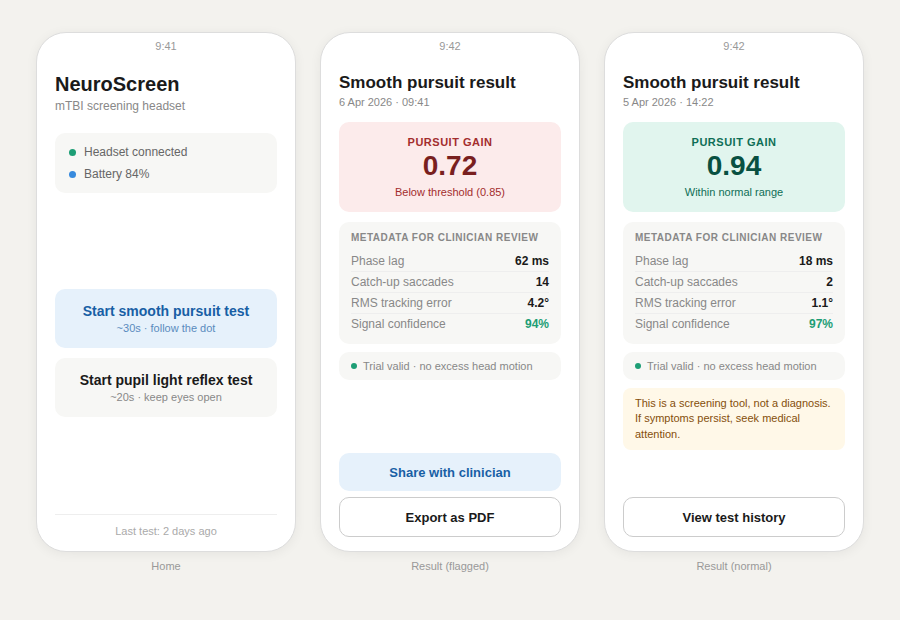
\includegraphics[width=\textwidth]{figures/app_design}
    \caption{App design for controlling the headset.}
    \label{fig:app-design}
\end{figure}

\section{On-Device Inference: LiteRT (formerly TensorFlow Lite) Runtime}

We decided on using LiteRT for the inference engine. A runtime shapes the system's latency, memory footprint, energy consumption, and operational reliability. Simultaneously running with the model are the stimulus display, IMU polling loop, Bluetooth communication, and the cameras. These system conditions paired with the fact that the models run entirely on the Pi~5 show that it is extremely important that an appropriate runtime is selected around our design choices and system philosophy.

The three inference backends evaluated for deploying MobileNetV2 on the Pi~5's Broadcom BCM2712 SoC were: PyTorch, ONNX Runtime, and LiteRT.

PyTorch was not selected as the inference engine since its main function is as a training and research framework rather than a lightweight inference engine. The PyTorch Pi tutorial shows that real-time inference on the Pi~5 is feasible, but considering it will be purely doing forward inference, the full framework is a heavier solution than necessary. ONNX Runtime, however, was intentionally engineered as an inference-focused runtime with a documented Raspberry Pi deployment path and an official edge tutorial, showing it to be a serious option~\cite{onnxruntime2021}.

This is further implied in research comparing the energy consumption of PyTorch versus LiteRT and ONNX Runtime~\cite{malenza2025energy}, showing that ONNX and LiteRT are more energy-efficient on MobileNetV2 for CPU workloads. This paper was on different hardware, however, so more specific benchmarking on the Pi~5 is needed to fully support this statement.

Furthermore, benchmarking on Pi ARM hardware shows that the runtime choice affects inference performance, with LiteRT performing strongly, especially when using INT8 quantisation~\cite{baller2021deepedgebench}. ONNX is frequently used in edge inference devices, with both LiteRT and ONNX being appropriate choices for inference on the Pi, with the final selection depending on future quantisation plans.

At FP32 inference the literature is ambiguous. This was resolved through benchmarking the runtimes on an Apple Silicon ARM CPU using four threads and FP32 precision to display approximately 1.2$\times$ better performance from LiteRT. Apple Silicon is not the Pi~5, with its cache hierarchy and SIMD width differing from the Cortex-A76 cores in the BCM2712, so the absolute latencies are not transferable and the relative rankings have their limitations too. Despite this, both use the ARM instruction set and these rankings are reinforced by trends seen in the literature~\cite{baller2021deepedgebench}.

\begin{table}[htbp]
    \centering
    \caption{Runtime benchmark comparison for MobileNetV2 FP32 inference on Apple Silicon ARM (4 threads, 200 passes, 30-iteration warmup).}
    \label{tab:runtime-benchmark}
    \begin{tabular}{lcccc}
        \toprule
        \textbf{Runtime} & \textbf{Mean Latency} & \textbf{P95} & \textbf{FPS} & \textbf{Model Size} \\
        \midrule
        \textbf{LiteRT (TFLite)} & \textbf{2.68\,ms} & 2.85\,ms & 373 & 11.5\,MB \\
        ONNX Runtime             & 3.23\,ms           & 3.82\,ms & 309 & 0.3\,MB \\
        PyTorch                  & 22.35\,ms          & 23.71\,ms & 45 & 12.0\,MB \\
        \bottomrule
    \end{tabular}
\end{table}

\Cref{tab:runtime-benchmark} shows that LiteRT achieves the best performance. Based on these results and the potential for future INT8 quantisation, LiteRT was selected as the more future-proof choice.

\subsection{Future Improvement and Current Limitations}

The present software uses FP32 deployment to avoid introducing quantisation errors in the gaze estimation pipeline. A future optimisation could be INT8 quantisation, which would cause the CPU inference efficiency to increase as the model size would reduce by approximately $4\times$. Further consideration would have to be put in how quantisation is done, as in MobileNet architectures post-training quantisation (PTQ) can cause large accuracy degradation~\cite{yun2021mobilenets}, whereas quantisation-aware training (QAT) is specifically designed for preserving accuracy~\cite{google_qat} by exposing the model to the effects of quantisation during the training process. This shows that although INT8 quantisation is attractive for constrained resources, the accuracy penalty must be properly controlled via careful quantisation methods. FP32 was therefore chosen for simplicity to achieve validation, with future software updates possibly including INT8 QAT optimisation. This reflects the intentions of the engineering philosophy concerning a simple and reliable baseline, where further optimisations can be brought in later.

\section{Smooth Pursuit Trial}

Smooth pursuit eye movement issues can occur with mTBI, as discussed in depth in \Cref{chapter:background}. Smooth pursuit dysfunction is a reliable indicator for underlying mTBI issues and specifically causes:

\begin{enumerate}
    \item \textbf{Saccadic jumps:} the eyes fall behind the object being watched and then jump forward to catch up.
    \item \textbf{Latency:} a delay between when the object starts moving and when the eyes start to follow it.
\end{enumerate}

The software in this section implements the smooth pursuit assessment pipeline for the headset hardware. For this trial, the user must follow a moving marker on the display screen moving sinusoidally horizontally. The camera collects the images of the eye, and the gaze estimation is compared with the ground truth angle from the marker to develop a set of metrics to assess if there are underlying pursuit issues. If they have smooth pursuit issues, the latencies and saccadic jumps will appear. Strong software was developed to use the data collected from the sensors to train a robust machine learning model and filter the outputs during testing so that truthful metrics can be extracted, producing meaningful and reliable results.

\subsection{Smooth Pursuit Metrics}

The metrics that were chosen are:

\begin{enumerate}
    \item \textbf{Pursuit gain:} Calculated through taking the FFT of both signals, as the target motion is sinusoidal, analysing the amplitudes at the stimulus frequency. Gain is defined as Amplitude$_{\text{eye}}$ / Amplitude$_{\text{target}}$. This should be close to unity, with lower values suggesting poor performance~\cite{devillerssidani2023oculomotor}.

    \item \textbf{Catch-up saccade activity:} The algorithm first calculates the eye velocity from the gaze estimation signal and detects the saccades where the velocity exceeds a threshold, retaining only the events which occur whilst the eye is behind the target and the jump reduces the tracking error~\cite{devillerssidani2023oculomotor}.

    \item \textbf{RMS tracking error:} The root-mean-square difference between the measured eye angle and the expected target angle~\cite{kellar2018comparing}.

    \item \textbf{Motion validity and signal confidence:} The module also outputs two quality-related quantities. Motion validity is derived from IMU-based gating logic and indicates whether excessive head movement compromised the trial. Signal confidence reflects the reliability of the eye-tracking signal, derived from analysis of blur, blinking, and glare.

    \item \textbf{Lag:} Calculated through the cross-correlation between the gaze estimation and ground truth signal, finding the time offset which maximises the correlation peak. This is consistent with prior work in which pursuit lag is treated as a key parameter~\cite{devillerssidani2023oculomotor}.
\end{enumerate}

These metrics are used to determine trial validity. The trial is disqualified if the IMU acceleration exceeds 1.5\,g for more than 300\,ms, or if more than 10\% of frames are rejected by the quality pipeline. These provisional thresholds will be revised against real headset data.

Gain was decided as the core metric for the trial result as it is the most clinically established metric~\cite{leigh2015neurology}, with the other metrics passed as metadata. The gain threshold was set at 0.85. At low stimulus frequencies ($\leq$0.4\,Hz), healthy horizontal pursuit gain is 0.9--1.0~\cite{meyer2020smoothpursuit}; 0.85 sits just below this range, giving noise tolerance without sacrificing sensitivity to genuine deficits. Metadata is provided so that clinicians can make more well-informed decisions about next steps, ensuring ethical considerations protect against false results such as false negatives.

\section{Data Collection Pipeline}

For training and testing, the data streams recorded are the display angle, the timestamps, the IMU motion stream, the quality indicators of the eye signal, and a signal derived from the eye. This derived signal is the raw eye image if collecting for training, and the predicted gaze angle if for testing.

The core difference is that in training mode the goal is to collect images of the eyes with the ground truth angle, and in testing, the goal is to collect the images of the eyes to determine an estimated gaze angle, comparing against the ground truth display angle to understand whether there are underlying smooth pursuit issues.

The data retention schemes for either are hence very different. In training, the system retains raw eye imagery together with the timeseries, event logs, and session metadata. Data is written locally in buffered chunks of 5~seconds, uploaded via WiFi due to system requirements, and then deleted shortly after to preserve memory. This was an engineering tradeoff as too long would mean a high risk of data loss if there is upload delay, and too frequent transfer would cause large transfer overhead.

In testing, the system stores the aligned timeseries, extracts the pursuit metrics, session metadata, and the final trial result, discarding the raw eye video after calculating the image confidence score and the estimated gaze angle. Image data is deleted as 120\,fps is storage intensive at approximately 2\,GB per 30-second session. The compact 5\,kB result is then transmitted to the user's phone via Bluetooth whilst caching the session summary until there is successful transfer, in case of sparse connectivity. Further evidence for this method is seen in research reflecting an edge-computing architecture where sensitive data is processed and stored locally first, with deferred bulk transfer used to reduce the real-time bandwidth and latency requirements so sensitive data is not transmitted over the network~\cite{rancea2024edge}.

Sustainability, IP, and security: These decisions were more environmentally friendly as edge computing is more carbon efficient than cloud computing~\cite{ma2025greening}. Immediately deleting the images and encrypting the wireless transmissions also help with minimising storage footprint and protecting the user's IP and security, under GDPR, CCPA, and HIPAA compliance. These principles can also be carried through in future iterations, extending useful life through keeping old practices.

\begin{figure}[htbp]
    \centering
    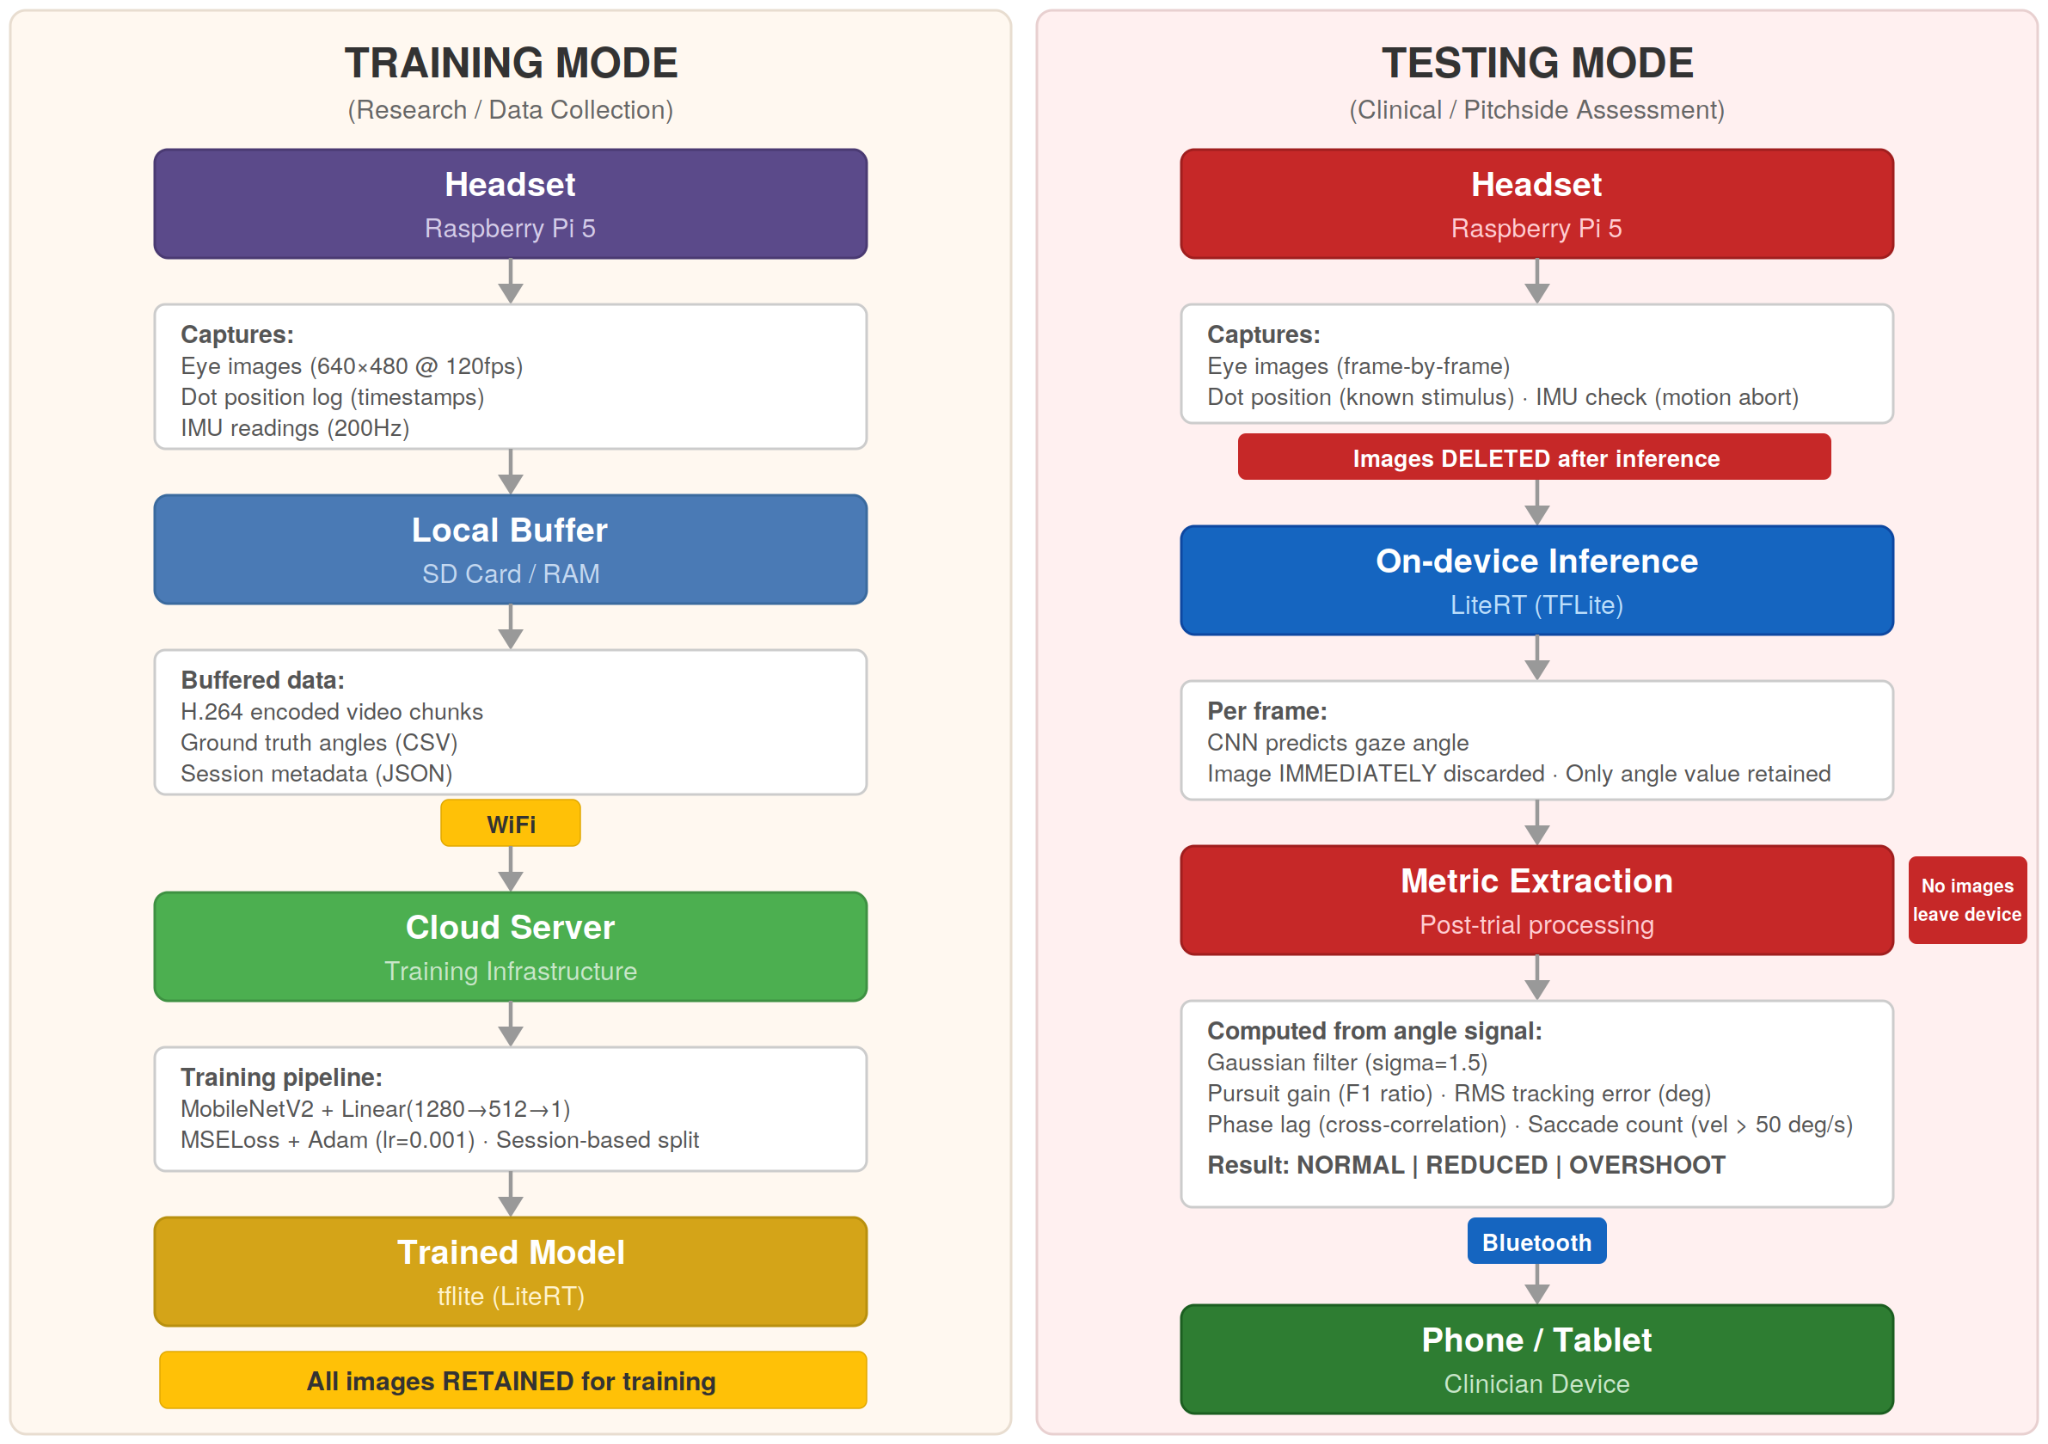
\includegraphics[width=\textwidth]{figures/data_pipeline}
    \caption{Data flow in the smooth pursuit trial, showing the training and testing paths.}
    \label{fig:data-pipeline}
\end{figure}

Both modes require synchronisation between the ground truth signal and the gaze estimation or image signal. In this prototype they are aligned through the monotonic software clock rather than by calibrating hardware latencies (sensor to CPU delay, screen render delay). Hardware calibration will be done in later hardware iterations.

\section{Testing Technologies}

When raw data is collected from the sensors and the gaze estimation model, it is important that it is cleaned so inference is accurate and the results are reliable. Regions of low confidence will exist in the gaze estimation due to blur, glare, and blinking. Removing these is important as they can poison metrics and give misleading results, carrying a risk of potential false negatives. Filtering is also necessary so that artifacts of noise which imitate poor pursuit performance are removed, letting us uncover the true gaze signal. This is predominantly saccade count as the noise imitates its characteristics, with catch-up saccade detection being the most noise-sensitive downstream metric~\cite{birawo2022review, leube2017sampling, cheng2026eye}. Unlike gain or RMS tracking error which are computed over longer temporal windows, the saccadic activity depends on brief high-velocity events and is therefore far more vulnerable to peaks. Simultaneously, over-filtering must be avoided as it can remove the original signal artifacts.

The model outputs gaze angles without confidence estimates; uncertainty-aware gaze regression is shown~\cite{kendall2017uncertainties, kuleshov2018accurate} to produce unreliable calibration, so image quality metrics such as blur and glare are used for external gating instead.

\subsubsection*{Blur and Blinking Detection}

The Laplacian of the image was analysed for detecting blur and blinking, having chosen a value of 1.6 as the cutoff with all values $\leq$~1.6 rejected. Blinking presents images similar to blur so the same algorithm is reused.

\begin{figure}[htbp]
    \centering
    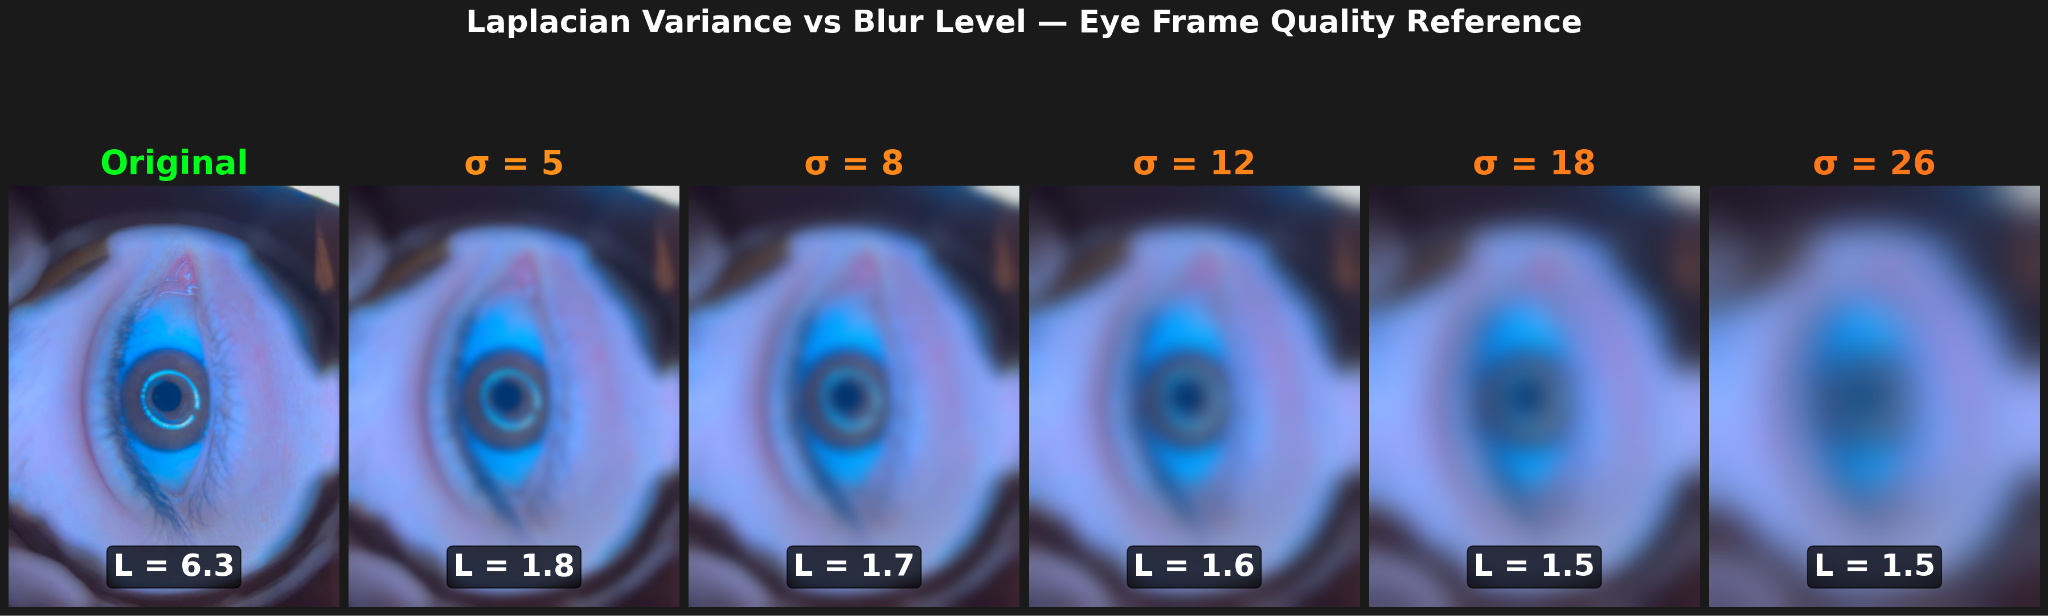
\includegraphics[width=\textwidth]{figures/blur_blink_detection}
    \caption{Blur and blinking---Laplacian variance vs blur level.}
    \label{fig:blur-blink}
\end{figure}

\subsubsection*{Glare Detection}

Glare detection involves analysing the saturated pixel ratio, choosing a value of 1\% as the cutoff so there is still room for glare whilst not poisoning our metrics, giving a balance of accuracy and practicality.

\begin{figure}[htbp]
    \centering
    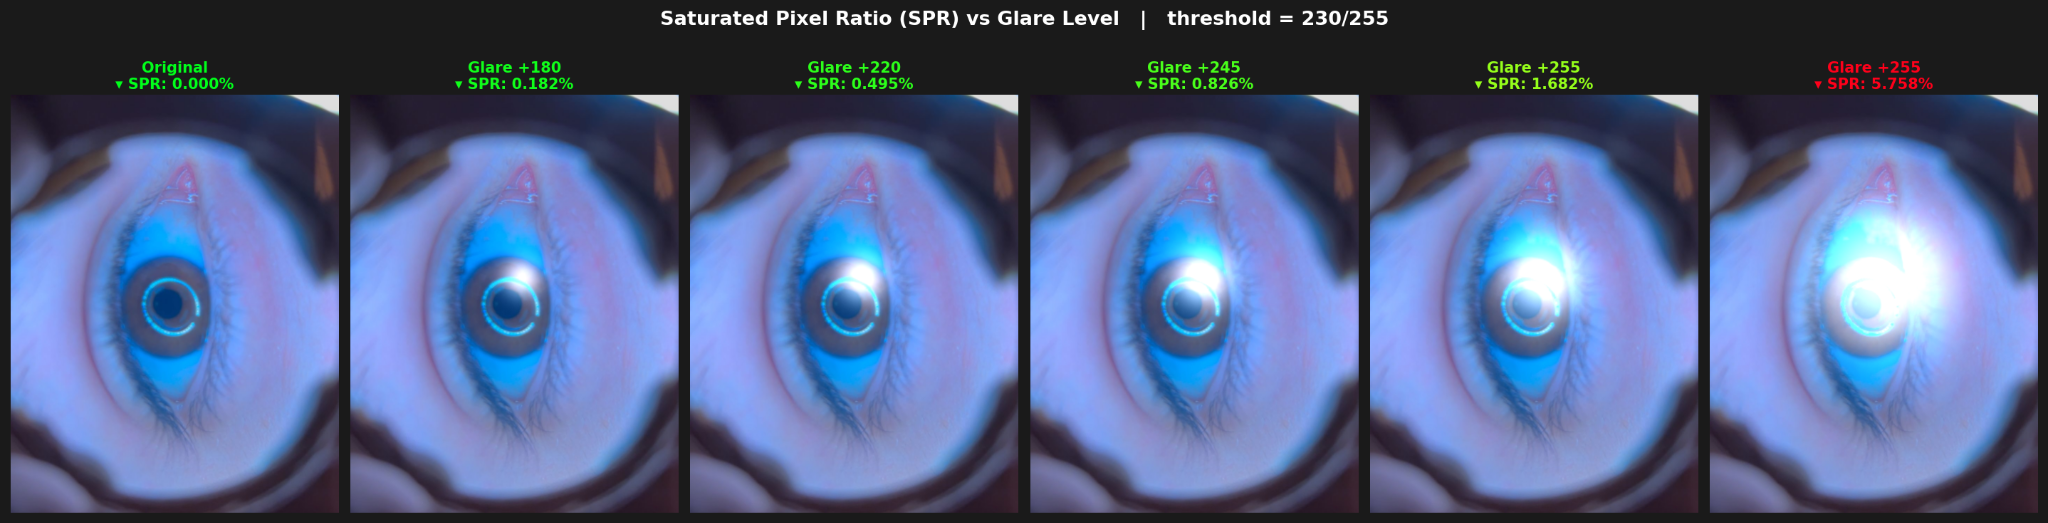
\includegraphics[width=\textwidth]{figures/glare_detection}
    \caption{Glare detection from 0\% to 5.758\% saturated pixel ratio.}
    \label{fig:glare}
\end{figure}

These thresholds outlined produced a risk mitigation strategy against false negatives, a dangerous failure mode prevented under ethical considerations.

\subsubsection*{Filter Selection}

The filter is to preserve genuine pursuit deficits whilst rejecting noise-induced artifacts. This methodology is validated on synthetic data so that the approach can be reused with real noise statistics once headset data is available. To fulfil this, synthetic pursuit trajectories were created from the ideal pursuit with no issues to the worst, increasing the saccade count each time. A comparison was then made between the true saccade count with the calculated one from the filtered signal to see which filter could reproduce the metrics most accurately, using sigma~$=$~0.6 noise addition between these as the test parameter. Saccades were used to guide the filter performance as it is the most noise-sensitive downstream metric, further supported in eye movement detection literature because saccades are detected using velocity-threshold algorithms~\cite{birawo2022review}, making them even more prone to noise after differentiation. Hence, this process was tuned against the most fragile part of the metric pipeline as the filter should then be adequate for the other slower, lower-frequency measures such as gain and RMS tracking error~\cite{birawo2022review}.

\begin{figure}[htbp]
    \centering
    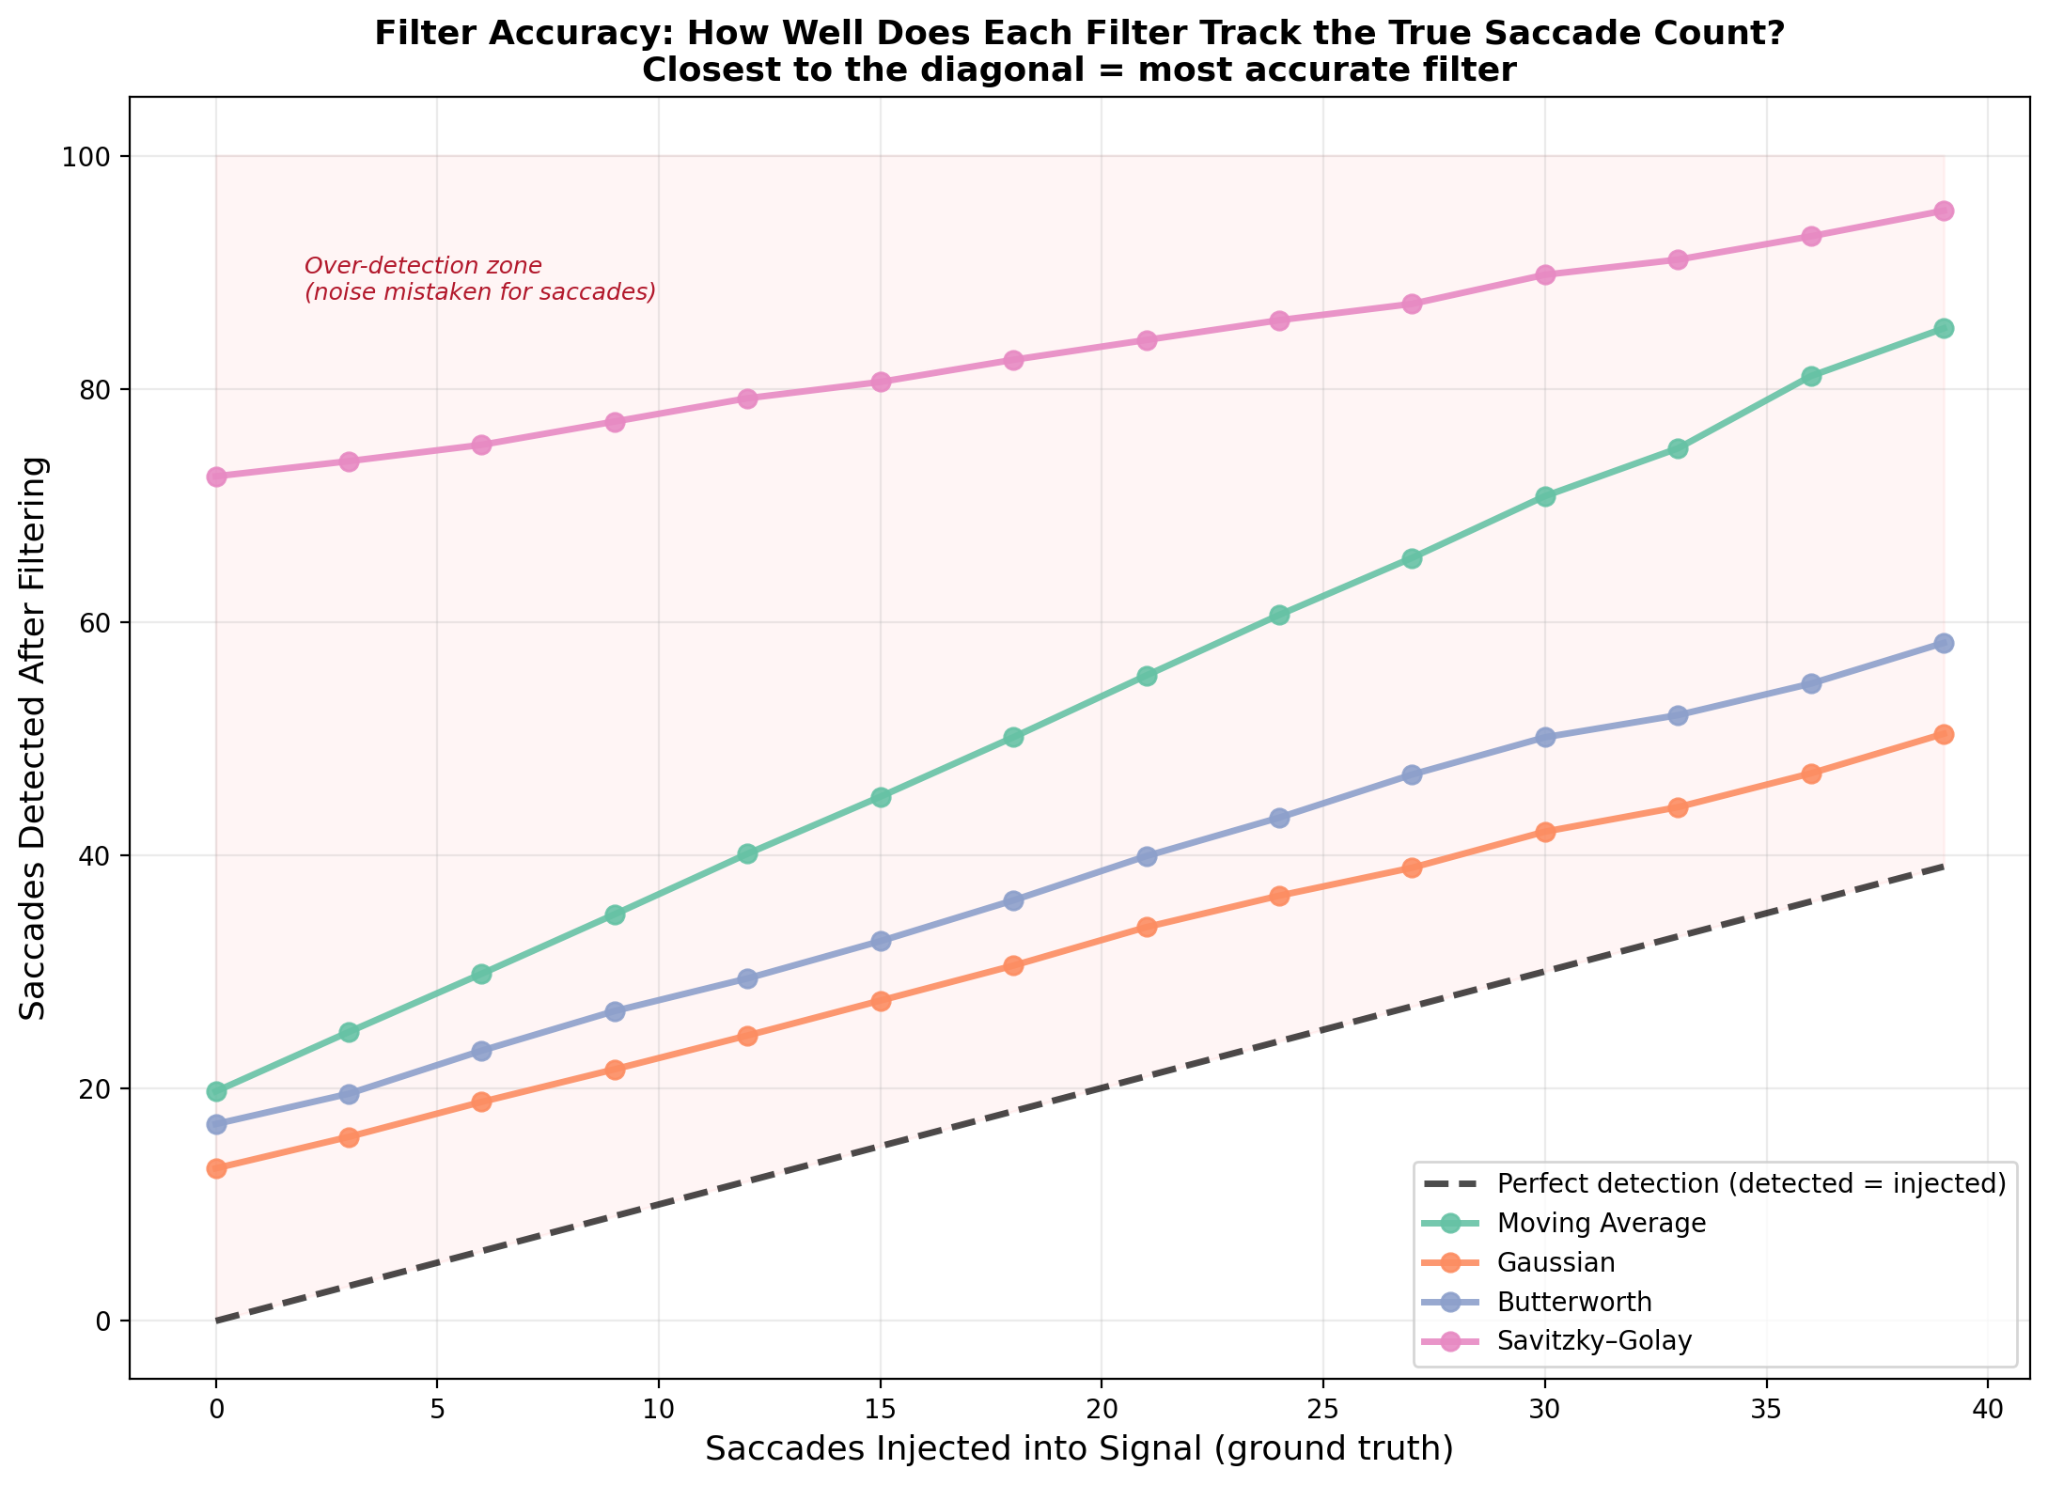
\includegraphics[width=\textwidth]{figures/filter_comparison}
    \caption{Gaussian filter performance comparison.}
    \label{fig:filter-comparison}
\end{figure}

\begin{figure}[htbp]
    \centering
    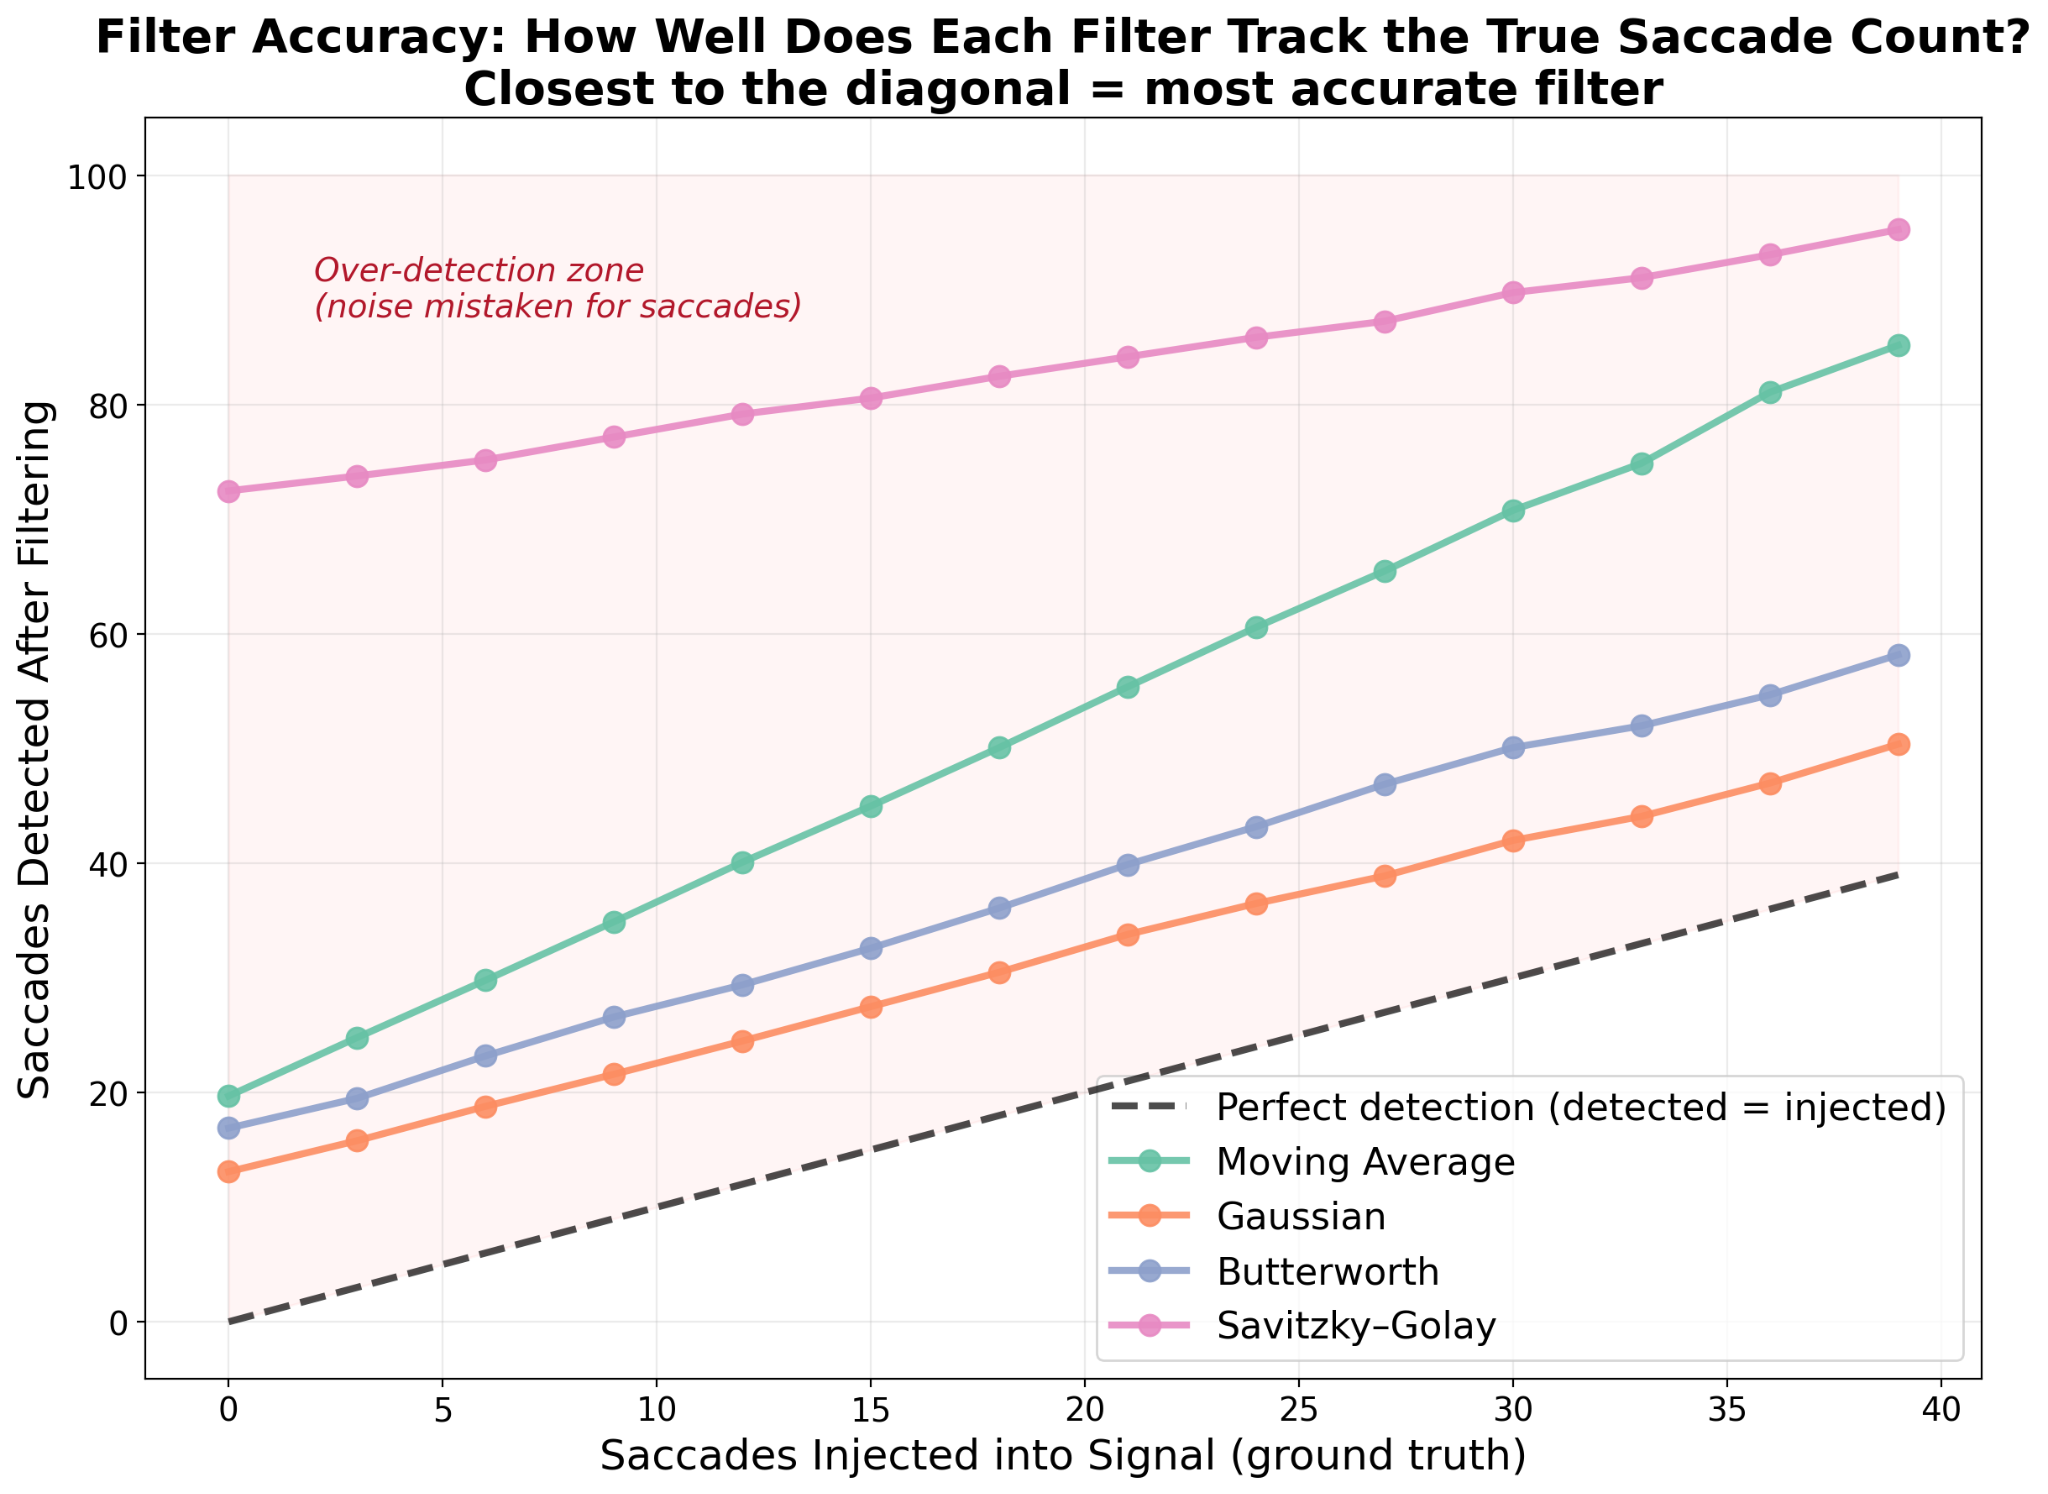
\includegraphics[width=\textwidth]{figures/gaussian_filter_optimisation}
    \caption{General filter performance comparison.}
    \label{fig:gaussian-optimisation}
\end{figure}

\Cref{fig:filter-comparison} shows that the Gaussian filter performs the best as it has the lowest error in saccade predictions. However, it still required optimisation, so a grid search was performed of the better Gaussian filters, achieving the filter in \Cref{fig:gaussian-optimisation}. The original unoptimised parameters were sigma~$=$~1.5 and threshold~$=$~30\,deg/s, giving MAE~$=$~12.2. Raising threshold to 50\,deg/s caught the real saccades, modelled as 120--240\,deg/s velocity peaks. These test results are evidence of the validity of this methodology.

\begin{figure}[htbp]
    \centering
    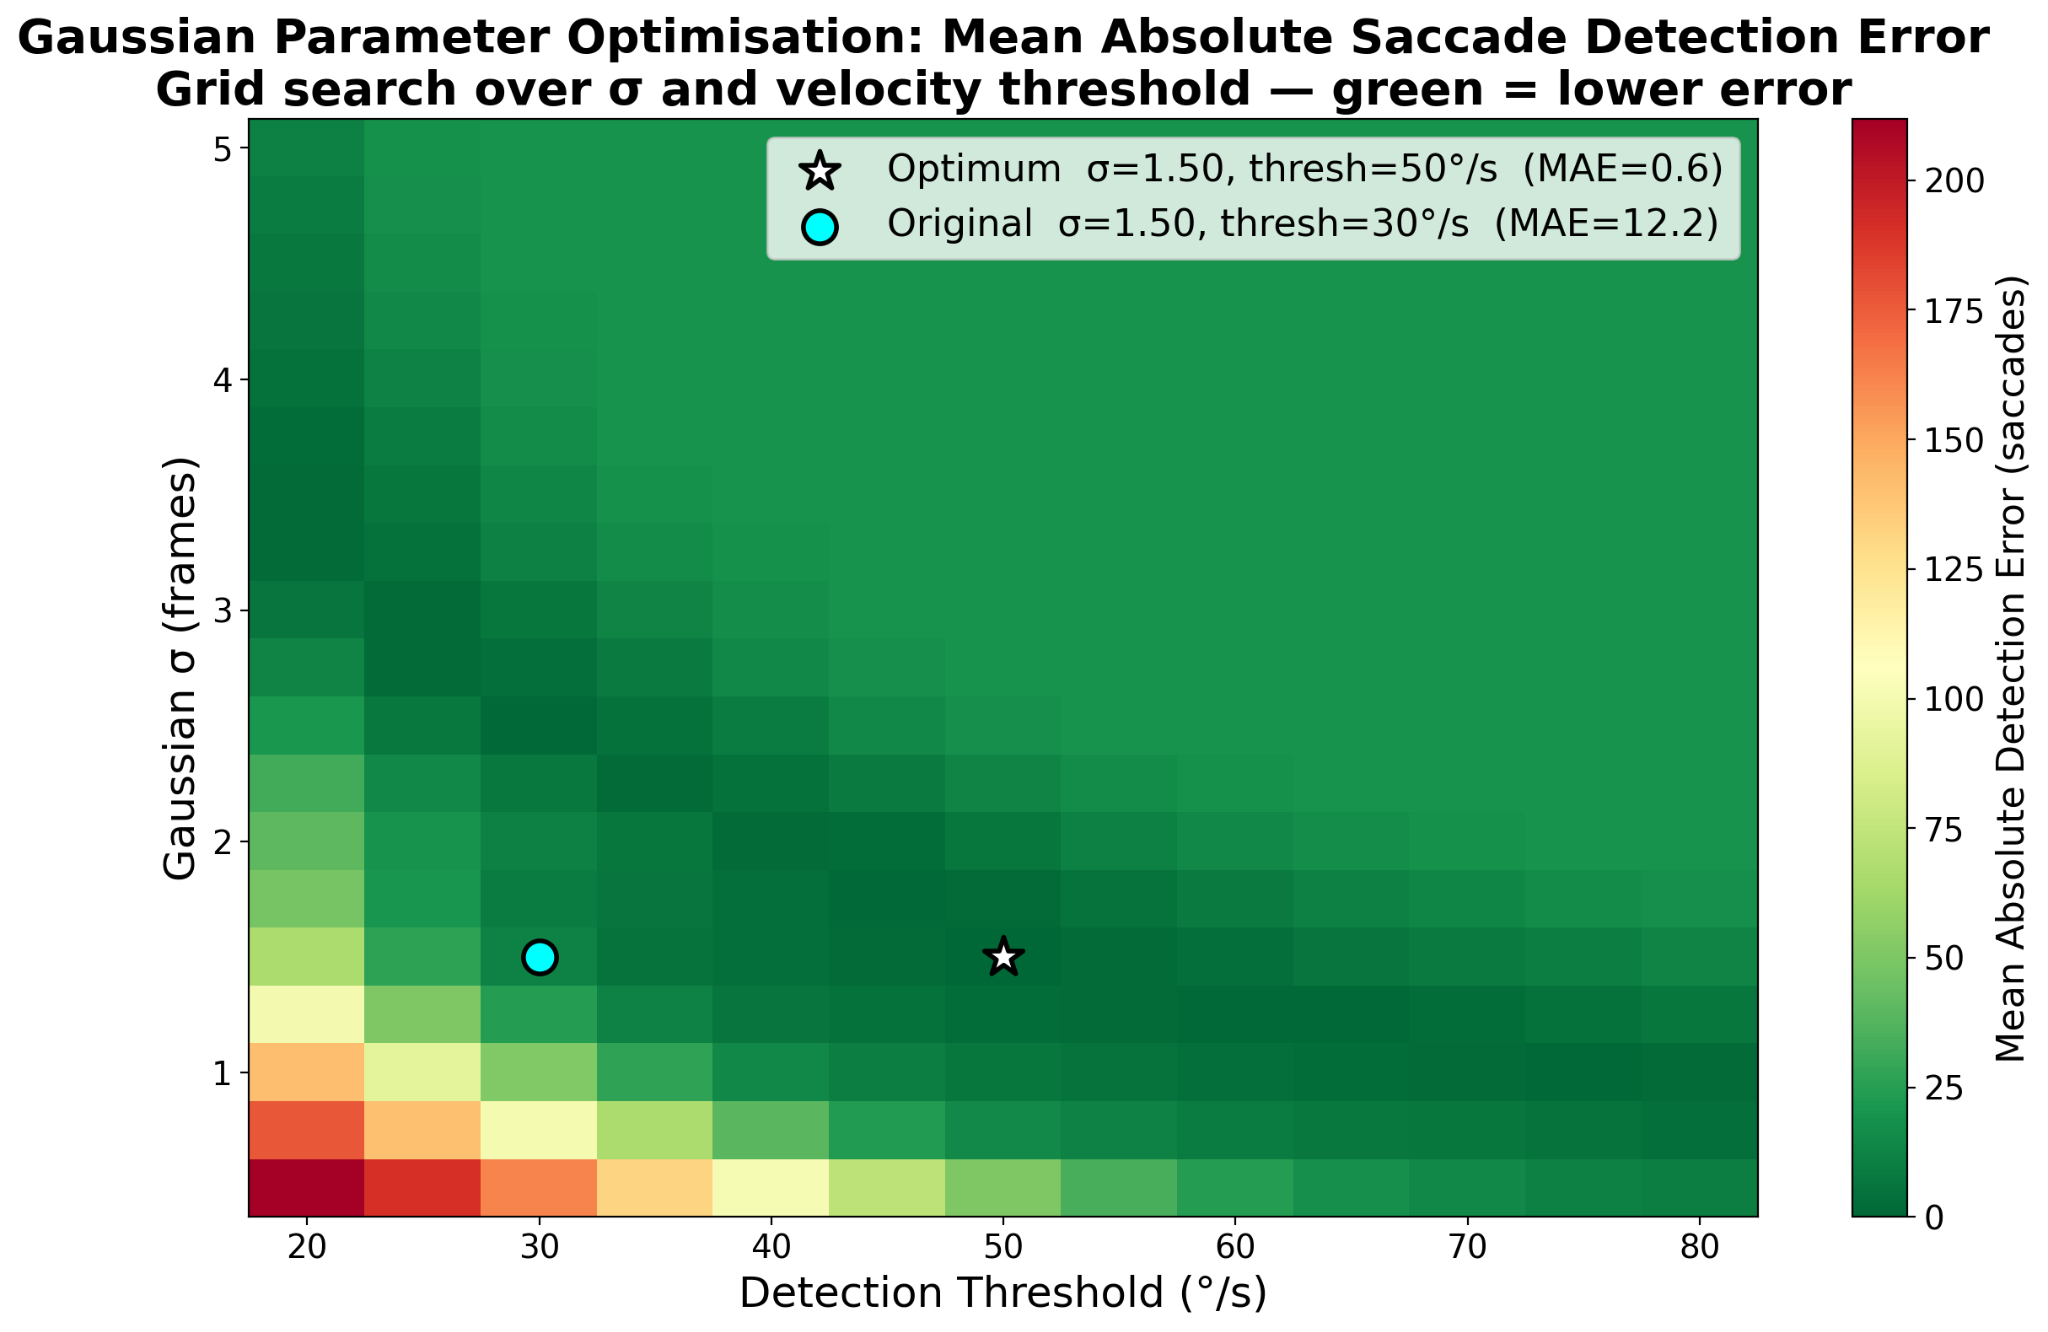
\includegraphics[width=\textwidth]{figures/optimal_gaussian_filter}
    \caption{Optimal Gaussian filter performance.}
    \label{fig:optimal-gaussian}
\end{figure}

\begin{figure}[htbp]
    \centering
    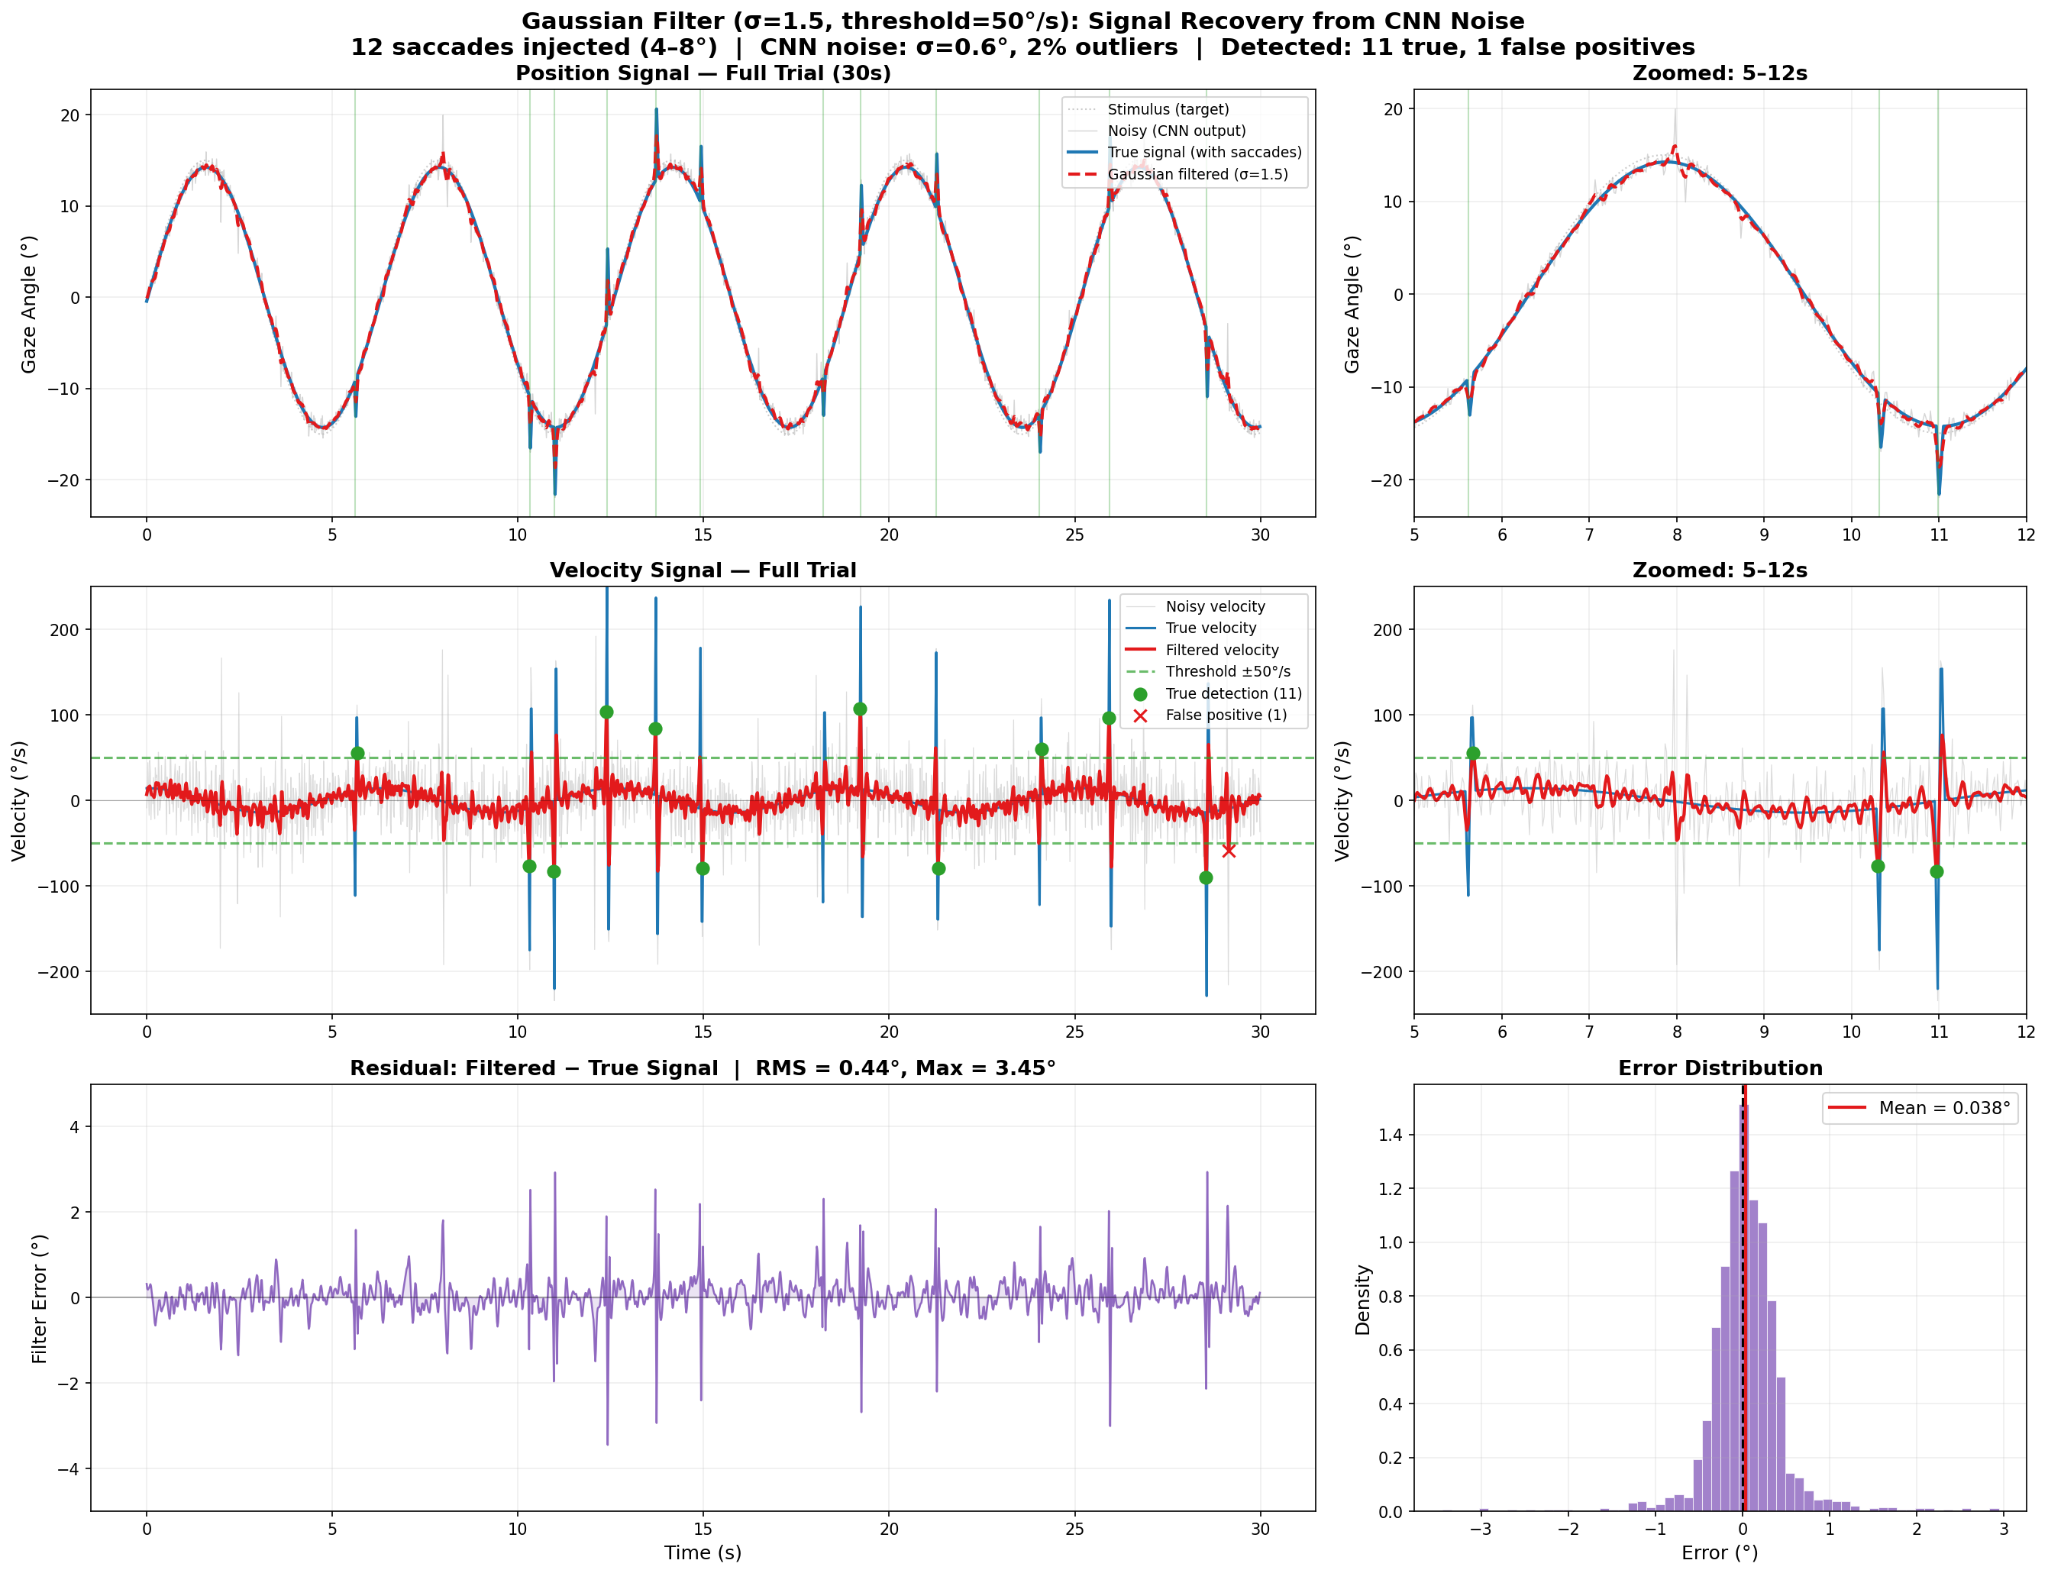
\includegraphics[width=\textwidth]{figures/filter_effects}
    \caption{Filter effects on a noisy signal.}
    \label{fig:filter-effects}
\end{figure}

\subsubsection*{Limitations and Future Improvements}

Saccades of 4--8 degrees of angular amplitude were injected for testing this filter, but there may be smaller ones that appear in future real headset data that would be harder to detect. This shows that the filter could be improved through using this same methodology further, iterating more in the future to provide the best filter for the end product. For now, this method has been proved and the parameters can be optimised later upon data collection, tuning noise and saccade amplitudes more appropriately. This is also the case for the glare, blurring, and IMU head shaking as further data collection is required to develop a more accurate threshold cutoff whilst using the same algorithms outlined in this section.

\section{Training Specific Technology}

The CNN used for understanding the gaze estimation was the MobileNetV2 model as it is explicitly designed for mobile and embedded vision workloads where inference must be fast and memory-efficient. Architectural features such as linear bottlenecks, inverted residual blocks, and depthwise separable convolutions reduce parameter count and the number of multiply-accumulate operations in comparison with heavier CNN alternatives, whilst still preserving useful representational capacity for strong feature understanding~\cite{sandler2018mobilenetv2}. This makes it a good fit for the Raspberry Pi~5 where the model is executed on the CPU whilst having to run camera capture, display update, logging, and Bluetooth/WiFi handling simultaneously. A plausible alternative would have been ResNet-18 as it is used widely for computer vision tasks, but it is computationally heavier than the MobileNetV2. Since this extra compute cost and power was not needed and we are optimising for faster and more efficient edge deployment, the MobileNetV2 was preferred over ResNet-18~\cite{he2016deep}.

The training process of the MobileNetV2 model was adapted to output the horizontal angle and achieve a low validation loss with strong generalisation. The pipeline was built and tested to show that the model structure is robust, so that when data is collected from the headset, the model can be trusted, leaving residual errors to be related to data needing further cleaning and augmentation. Methods are to be reused to automatically remove poor images from the dataset, using the confidence signals to remove poor data and prevent model corruption.

A custom regression head was applied as the MobileNetV2 classifier is designed for ImageNet classification rather than gaze-angle regression~\cite{sandler2018mobilenetv2}. The 1280-dimensional feature vector produced by the MobileNetV2 is then passed through the head which consists of Dropout ($p$~$=$~0.2), a linear reduction from 1280 to 512 dimensions, a ReLU activation, a second Dropout layer ($p$~$=$~0.2), and a final linear projection to the gaze-angle model.

ReLU and dropout layers are used to help prevent overfitting, for instance in subject-specific appearances~\cite{srivastava2014dropout}, supporting generalisation for new users and learning non-linear features of the data.

The backbone was fine-tuned from the start rather than freezing it as the domain gap between ImageNet photographs and the near-infrared eye images is large enough such that adaptation is needed beyond the final layers. This is consistent with the wider literature on transfer learning, showing that feature transferability decreases as the target tasks and input distribution diverge from the original pretraining domain~\cite{yosinski2014transferable}.

The loss function chosen was MSELoss which is optimal for 1D regression due to the continuous output with Gaussian noise~\cite{zhang2015appearance, krafka2016eye}. Both use MSE loss for gaze regression, showing this to be a conventional loss function for the task.

Adam~\cite{kingma2015adam} was selected as the optimiser with a learning rate of 0.001 for early testing, and SGD with momentum for once the hardware design has stabilised. Research found that SGD with momentum outperformed Adam in their eye tracking experiments~\cite{chugh2020eye}, achieving lower final validation loss despite the slower initial convergence. This result is also consistent with a broader finding in the optimisation literature where Adam will cause convergence to a sharp minima that generalises more poorly, whereas SGD's noisier gradient estimates usually have flatter minima with better generalisation~\cite{keskar2017large, wilson2017marginal}. Adam will be initially used, however, as the immediate need is using small amounts of collected data to reach stable and rapid convergence, where the model and preprocessing pipeline are still being iterated. A linear warmup schedule was also implemented that increased the learning rate from near-zero to the target value over the first 5 epochs. This was essential to do as the regression head is randomly initialised whilst the backbone carries the pretrained weights. Without the warmup, the large initial gradients from the head propagate backward and will destroy pretrained features before they have the opportunity to align with the new task. After the warmup, a ReduceLROnPlateau scheduler halves the learning rate if the validation loss stalls for 5 consecutive epochs.

\subsection{Architecture Validation on MPIIGaze}

To validate that these are sensible choices for a machine learning architecture independently of the headset hardware, the pipeline was evaluated on the MPIIGaze benchmark~\cite{zhang2015appearance}, a popular public dataset containing 213{,}659 normalised eye patches from 15 subjects with calibrated 3D gaze direction labels. Training was performed on NVIDIA A100 GPUs and a leave-one-person-out cross validation so that all the images from one subject are kept for testing whilst keeping the remaining 14 subjects for the training set. This is important as it ensures that the validation accuracy reflects true cross-subject generalisation. By showing a competitive accuracy on a known benchmark, this can show that errors in the headset model can be attributed to the headset domain-specific factors in its data collection such as camera resolution and viewing geometry, rather than issues with the model architecture and optimiser set out above. For robustness, both optimisers were used in this comparison.

\begin{table}[htbp]
    \centering
    \caption{15-fold LOPO cross-subject evaluation on MPIIGaze. Our pipeline matches published baselines with a substantially lighter backbone chosen for edge deployment on the Raspberry Pi.}
    \label{tab:mpiigaze-results}
    \begin{tabular}{lccc}
        \toprule
        \textbf{Method} & \textbf{Backbone} & \textbf{Test MAE (15-fold)} \\
        \midrule
        Zhang et al.~\cite{zhang2015appearance} & AlexNet-based & 6.3\textdegree{} \\
        Zhang et al.~\cite{zhang2017appearance} & ResNet-based & 4.80\textdegree{} \\
        Cheng et al.~\cite{cheng2018appearance} & Evaluation-guided asymmetric & 4.70\textdegree{} \\
        Ours (Adam) & MobileNetV2 (11.5\,MB) & 4.97\textdegree{} \\
        Ours (SGD) & MobileNetV2 (11.5\,MB) & 4.85\textdegree{} \\
        \bottomrule
    \end{tabular}
\end{table}

The pipeline achieved 4.97\textdegree{} (Adam) and 4.85\textdegree{} (SGD) mean MAE across the 15 folds, which is competitive with Cheng et al.\ (4.70\textdegree{}), Zhang et al.\ 2017 (4.80\textdegree{}), and 2015 (6.3\textdegree{}). This benchmark validates that the choices of training loop, loss function, and architecture are not the main limiting factor for gaze regression and that the residual error on the headset data is more strongly associated with domain-specific factors such as geometry, subject variance, and IR imagery. Therefore, future optimisations should consider data quality, labelling, and IR-specific augmentation whilst not excluding architecture-specific choices, but rather putting them as a secondary concern instead.

\section{Summary and Design Considerations of the Smooth Pursuit Trial}

The smooth pursuit software developed in this section has met the constraints identified including: GDPR, HIPAA, and CCPA compliance through image deletion; methodologies that are reusable and can be tuned further in the future (synthetic filter validation with MAE 0.6 saccades, architecture validation, basis thresholds); running on the Pi~5 with LiteRT achieving 2.68\,ms mean inference latency with the concurrent display and sensor workloads; developing a training pipeline that displays competitive metrics at 4.97\textdegree{} against literature values such as Cheng et al.\ (4.70\textdegree{}), Zhang et al.\ 2017 (4.80\textdegree{}), and 2015 (6.3\textdegree{}).

The main limitation throughout, however, is the lack of real headset data. This includes filter thresholds, quality gates, and IMU validity cutoffs which are provisional but can be rechosen using the same methodologies once the data becomes available. Architectural changes have not been completely struck off but are less of a concern in comparison with labelling quality, subject diversity, and IR-specific augmentation given the MPIIGaze results. The next steps should be headset data collection, thresholding retuning, and selecting a final optimiser.


\section{Pupil Width Estimation}
\label{sec:pupil-width}

This section describes the pipeline that converts raw eye images from the headset camera into \ab{plr} biomarker measurements. The pipeline must satisfy the following requirements, derived from the literature review  (\Cref{chapter:background}) and the headset hardware (\Cref{chapter:headset}):

\begin{itemize}
    \item \textbf{Precision.} Resolve the pupil diameter changes associated with \ab{plr} abnormalities in \ab{mtbi}, which manifest as differences of 15--20\% in constriction amplitude and 15--20\,ms in latency between concussed and healthy populations;~\cite{master2020pupillary, ciuffreda2017plr}).

    \item \textbf{Robustness.} Handle blinks (100--400\,ms of complete data loss) and other transient artefacts gracefully, detecting and discarding corrupted frames rather than propagating erroneous measurements.

    \item \textbf{Ease of use.} Operate without specialist training or equipment, producing measurements that are comparable across subjects.

    \item \textbf{Inference.} Complete processing within the 8.3\,ms per-frame budget imposed by the headset's 120\,fps capture rate on the Raspberry Pi~5.

\end{itemize}


\subsection{Pipeline Design}
\label{sec:pipeline}

\begin{figure}[htbp]
    \centering
    
\includegraphics[width=\textwidth]{pipeline_figure.pdf}
    \caption{Pupil width estimation pipeline overview. (a)~Preprocessing: raw eye images undergo contrast enhancement. (b)~Direct regression: a CNN predicts pupil diameter as a single scalar. (c)~Semantic segmentation: a CNN produces per-pixel class labels from which iris and pupil boundaries are extracted via ellipse fitting, yielding multiple outputs including confidence. (d)~Biomarker extraction: per-frame measurements are accumulated into a time series and fitted with a parametric PLR model to extract clinically relevant biomarkers.}
    \label{fig:pipeline}
\end{figure}

Two approaches dominate the recent literature for learning-based pupil measurement. In a \emph{regression} approach, a model predicts ellipse parameters directly from the raw image~\cite{kothari2021ellseg, jia2024condseg}. In a \emph{segmentation} approach, the model classifies each pixel into anatomical regions (pupil, iris, sclera, background) and an ellipse is fitted to the segmented boundary~\cite{chaudhary2019ritnet}.

We adopt segmentation. On \textbf{accuracy}, recent comparative work shows complementary strengths: regression achieves tighter ellipse centre localisation (1.12 vs 1.47\,px on OpenEDS), while segmentation produces higher-quality boundaries (97.4\% vs 94.6\% iris \ab{iou})~\cite{jia2024condseg, kothari2021ellseg}. Since our downstream task (tracking diameter changes over time) depends on boundary precision rather than absolute centre accuracy, segmentation is slightly better suited.

On \textbf{robustness}, segmentation produces a per-pixel probability map from which we derive per-frame confidence scores for automated quality gating: frames where the model is uncertain are downweighted or discarded before biomarker extraction, preventing corrupted measurements from propagating downstream. Regression provides no equivalent signal. On \textbf{interpretability}, the segmentation mask is directly inspectable: when the pipeline reports an anomalous \ab{plr} measurement, a user or developer can examine the mask to determine whether the anomaly reflects a genuine physiological response or a processing artefact.

The trade-off is \textbf{annotation cost} when adapting to new hardware. Pixel-level segmentation masks require minutes per image to produce, whereas regression labels (e.g.\ clicking two points on the pupil boundary) take seconds, making regression substantially cheaper to fine-tune on a new device. We offset this by training on existing datasets (OpenEDS; 12\,759 masks~\cite{garbin2019openeds}), applying domain-specific augmentation (\Cref{sec:domain-transfer}), and validating end-to-end using cheaply acquired regression-style diameter labels from our headset.

For a screening tool whose output may prompt referral to a medical professional, the robustness and interpretability advantages take priority over annotation cost: silent failures risk missed referrals, and the ability to audit predictions is essential for trust in the system's output. \Cref{tab:design-matrix} summarises the comparison.

\begin{table}[htbp]
\centering
\caption{Design comparison for pupil diameter extraction. \textbf{Bold} indicates the stronger approach for each criterion.}
\label{tab:design-matrix}
\begin{tabular}{l c c}
\toprule
\tableHCell{Criterion} & \tableHCell{Regression} & \tableHCell{Segmentation} \\
\midrule
Accuracy            & \multicolumn{2}{c}{Complementary (see text)} \\
Robustness          & No per-frame confidence & \textbf{Probability map} \\
Interpretability    & Opaque                  & \textbf{Inspect mask} \\
Annotation cost     & \textbf{Seconds/image}  & Minutes/image \\
Real-time inference & \multicolumn{2}{c}{Both feasible at 120\,fps} \\
\bottomrule
\end{tabular}
\end{table}

\subsection{Ablation}
\label{sec:ablation}

Within the segmentation pipeline, three factors must be configured: model architecture, loss function, and preprocessing. We ablate each on the OpenEDS benchmark to verify our choices. As shown in \Cref{tab:baseline-results}, performance is saturated across architecture and loss function choices; preprocessing is the only ablated factor that meaningfully affects accuracy.

All models are trained on OpenEDS~\cite{garbin2019openeds} (12\,759 annotated images, 152 participants) with the Adam optimiser (learning rate $10^{-3}$), ReduceLROnPlateau scheduling, for 50 epochs on an NVIDIA RTX A4000 (16\,GB). Due to compute constraints, we run three seeds for one configuration per architecture (RITnet + Dice, U-Net + CE) to characterise run-to-run variance, and single seeds for the remaining configurations.

\paragraph{Architecture.} Deployment on the headset's Raspberry Pi~5 imposes inference compute constraints (the 8.3\,ms per-frame budget at 120\,fps has not yet been verified on-device). We compare RITnet~\cite{chaudhary2019ritnet}, a lightweight DenseNet--U-Net hybrid (250K parameters, {<}1\,MB), against a standard U-Net (7.8M parameters, 29.6\,MB). As \Cref{tab:baseline-results} shows, both architectures achieve comparable pupil axis error (0.09 vs 0.13 $\pm$ 0.02\,px), but U-Net is 46\% slower and 30$\times$ larger.

\paragraph{Loss function.} Not all pixels matter equally for diameter estimation: accuracy depends on the pupil--iris boundary. We compare cross-entropy, generalised Dice (which addresses class imbalance by weighting each class inversely by area), CE + Dice, and a compound loss adding a boundary-aware term that upweights pixels near class edges~\cite{chaudhary2019ritnet}. The spread in axis error across all four is 0.04\,px (\Cref{tab:baseline-results}), comparable to the $\pm$0.03\,px seed-to-seed variance observed for Dice. Since the differences are within noise, we adopt the compound loss following the original RITnet paper: the boundary-aware term is theoretically motivated for our boundary-sensitive task, even though its empirical effect is small at this dataset scale.

\paragraph{Preprocessing.} Raw eye images exhibit low contrast between iris and pupil. We apply gamma correction ($\gamma = 0.8$, a nonlinear intensity mapping that brightens dark regions) and CLAHE (contrast-limited adaptive histogram equalisation; clip limit 1.5, tile grid $8 \times 8$), which enhances local contrast without amplifying noise globally. Removing both approximately triples axis error (0.10 to 0.32\,px), making preprocessing the only factor with a meaningful effect.

\begin{table}[htbp]
\centering
\caption{Configuration ablation on the OpenEDS test set. $^\dagger$Mean $\pm$ SD across 3 seeds. FPS measured on an NVIDIA RTX A4000.}
\label{tab:baseline-results}
\begin{tabular}{l l l r r r r}
\toprule
\tableHCell{Model} & \tableHCell{Loss} & \tableHCell{Preproc.} & \tableHCell{Pupil IoU (\%)} & \tableHCell{Axis err (px)} & \tableHCell{Size (MB)} & \tableHCell{FPS} \\
\midrule
RITnet & CE              & Yes & 98.76 & 0.10 & 1.07 & 160 \\
RITnet & Dice$^\dagger$  & Yes & 98.91 $\pm$ 0.02 & 0.12 $\pm$ 0.03 & 1.07 & 167 $\pm$ 10 \\
RITnet & CE + Dice       & Yes & 98.98 & 0.08 & 1.07 & 188 \\
\textbf{RITnet} & \textbf{Compound} & \textbf{Yes} & \textbf{98.93} & \textbf{0.09} & \textbf{1.07} & \textbf{148} \\
RITnet & CE              & No  & 97.82 & 0.32 & 1.07 & 226 \\
U-Net$^\dagger$  & CE    & Yes & 98.93 $\pm$ 0.10 & 0.13 $\pm$ 0.02 & 29.6 & 130 $\pm$ 3 \\
\bottomrule
\end{tabular}
\end{table}

We select RITnet with compound loss and gamma+CLAHE preprocessing as the deployment configuration (bold in \Cref{tab:baseline-results}).

\subsection{Domain Transfer}
\label{sec:domain-transfer}

\paragraph{Domain gap.} OpenEDS was collected using a research-grade eye tracker with near-infrared illumination, high-resolution optics, and controlled viewing geometry. The headset uses \todo{fill in camera details from electronics section} viewing through a beamsplitter under display-reflected visible light. \Cref{fig:domain-gap} illustrates the visual differences: the headset images are lower resolution, exhibit different contrast characteristics, and contain reflections from the beamsplitter optics.

\begin{figure}[htbp]
    \centering
    \begin{minipage}{0.35\textwidth}
        \centering
        
\includegraphics[width=\textwidth]{raw_eye_crop}
        \subcaption{OpenEDS (research eye tracker)}
    \end{minipage}
    \hfill
    \begin{minipage}{0.35\textwidth}
        \centering
        
\includegraphics[width=\textwidth]{headset_raw_cropped}
        \subcaption{Headset}
    \end{minipage}
    \caption{Domain gap between training data and deployment hardware. The images differ in resolution, contrast, illumination spectrum, and noise characteristics.}
    \label{fig:domain-gap}
\end{figure}

\paragraph{Augmentation strategy.} Annotating pixel-level segmentation masks for headset images is prohibitively labour-intensive (as discussed in \Cref{sec:pipeline}). Instead, we bridge the domain gap through data augmentation that simulates the headset imaging conditions during training. We evaluate two strategies of increasing specificity, with results in \Cref{tab:augmentation-results}.

\emph{Standard augmentation} applies geometric transforms (random horizontal flips, small rotations) and photometric perturbations (brightness, contrast, and Gaussian noise jitter) that improve generalisation across any target domain.

\emph{Domain-specific augmentation} adds transforms targeting the identified differences: sclera region brightening (simulating the different illumination balance), resolution downsampling (matching the headset's lower effective resolution), and blur (simulating slight defocus through the beamsplitter optics).

\begin{table}[htbp]
\centering
\caption{Effect of augmentation on OpenEDS test set performance and headset pupil detection rate. Augmentation reduces OpenEDS accuracy (as expected, since the training distribution is broadened) but dramatically improves headset generalisation.}
\label{tab:augmentation-results}
\begin{tabular}{l r r r}
\toprule
\tableHCell{Configuration} & \tableHCell{Pupil IoU (\%)} & \tableHCell{Axis err (px)} & \tableHCell{Headset detection (\%)} \\
\midrule
No augmentation (baseline)  & 98.93 & 0.09 & 22.1 \\
Standard augmentation       & 98.19 & 0.23 & \todo{--} \\
Domain-specific augmentation & 79.28 & 2.68 & 52.3 \\
Domain-specific + 112$\times$112 & 92.72 & 0.27 & \todo{--} \\
\bottomrule
\end{tabular}
\end{table}

The domain-specific augmentation at full OpenEDS resolution significantly degrades in-distribution performance (pupil \ab{iou} drops to 79.3\%) because the aggressive transforms push the training distribution far from the OpenEDS test set. Training at the headset's native resolution (112$\times$112) partially recovers OpenEDS performance (92.7\% \ab{iou}) while maintaining the domain adaptation benefit. On headset images, domain-specific augmentation increases pupil detection from 22\% to 52\%, with sensible diameter measurements (pupil/iris ratio $0.45 \pm 0.09$) where the baseline model produces largely invalid fits.

\paragraph{Headset validation.} \Cref{fig:headset-validation} shows segmentation overlays on headset-captured images for the baseline and domain-augmented models. The baseline model frequently fails to segment the pupil or produces fragmented predictions, whereas the domain-augmented model achieves coherent segmentation on the majority of frames where the pupil is visible. \todo{Add regression-label diameter comparison on ${\sim}100$ labelled headset frames.}

\begin{figure}[htbp]
    \centering
    \begin{minipage}{0.48\textwidth}
        \centering
        
\includegraphics[width=\textwidth]{headset_baseline_overlay}
        \subcaption{Baseline model (22\% detection)}
    \end{minipage}
    \hfill
    \begin{minipage}{0.48\textwidth}
        \centering
        
\includegraphics[width=\textwidth]{headset_domain_aug_overlay}
        \subcaption{Domain-augmented model (52\% detection)}
    \end{minipage}
    \caption{Segmentation results on headset-captured images. The baseline model (a) produces fragmented, mostly invalid predictions. Domain-specific augmentation (b) yields coherent pupil and iris segmentation on the majority of frames where the eye is visible.}
    \label{fig:headset-validation}
\end{figure}


\subsection{PLR Biomarker Extraction}
\label{sec:plr-extraction}

This subsection describes how per-frame segmentation masks are converted into clinically relevant \ab{plr} biomarkers. Each step is presented alongside the evidence that it works.

\paragraph{Diameter extraction.} Given a segmentation mask, we fit an ellipse to the largest pupil contour via least squares, yielding centre coordinates, major and minor axis diameters, and rotation angle. We report mean diameter (average of major and minor axes) for robustness to foreshortening from small head rotations within the headset.

The standard approach applies \texttt{argmax} to the segmentation logits before fitting, discarding the model's uncertainty. We improve on this with a probability-weighted fit: each pixel's contribution is weighted by its softmax probability of belonging to the pupil class, so uncertain boundary pixels have less influence than confident interior pixels. \todo{Report axis error improvement: hard vs soft fitting on OpenEDS test set.}

We normalise pupil diameter by the simultaneously measured iris diameter, producing a dimensionless pupil--iris ratio. Adult iris diameter varies by only ${\sim}3.4\%$ across individuals (11.8\,mm $\pm$ 0.4\,mm~\cite{boyle2021hvid}), so this ratio reflects true pupil size changes rather than geometric scaling, removing the need for per-subject calibration.

\paragraph{Signal cleaning.} The raw diameter time series contains frame-to-frame jitter, data gaps from blinks, and low-frequency pupil oscillations (hippus, 0.5--2\,Hz). Three steps clean the signal before biomarker extraction. \textbf{Blink detection:} frames where the pupil area drops below 50\% of the pre-stimulus baseline or where the segmentation confidence falls below a threshold are identified; short blinks are interpolated, while blinks during the constriction phase invalidate the trial. \textbf{Outlier rejection:} frames where the frame-to-frame diameter change exceeds 8\,mm/s (approximately mean + 2\,SD of healthy peak constriction velocity~\cite{bremner2012pupillometric}) are treated as segmentation failures and interpolated. \textbf{Savitzky--Golay filtering:} a local polynomial is fitted to each window for temporal smoothing~\cite{savitzky1964smoothing}. Unlike a Gaussian kernel, this preserves the sharp constriction onset that is critical for accurate peak velocity estimation.

\paragraph{Parametric curve fitting.} Rather than extracting biomarkers from local derivatives of the smoothed signal (which amplify noise), we fit a parametric model to the entire post-stimulus waveform~\cite{fan2011modeling}:
%
\begin{equation}
    d(t) = d_0 - A \left(1 - e^{-(t - t_{\mathrm{onset}})/\tau_c}\right) e^{-(t - t_{\mathrm{onset}})/\tau_d}
    \label{eq:plr-model}
\end{equation}
%
where $d_0$ is the baseline diameter, $A$ is the constriction amplitude, $t_{\mathrm{onset}}$ is the latency, $\tau_c$ is the constriction time constant, and $\tau_d$ is the dilation recovery time constant. The model is fitted via nonlinear least squares with physiologically informed bounds on each parameter. This acts as a physics-informed regulariser: every data point contributes to every parameter estimate, and the model rejects solutions that would correspond to impossible pupil dynamics. The fitted parameters directly yield the clinically relevant biomarkers identified in \Cref{chapter:background}: constriction latency ($t_{\mathrm{onset}}$), constriction amplitude ($A/d_0 \times 100\%$), peak constriction velocity ($\max |d'(t)|$, derivable analytically), and recovery time constant ($\tau_d$). \Cref{fig:plr-fitted} shows an example fit.

\begin{figure}[htbp]
    \centering
    
\includegraphics[width=0.85\textwidth]{plr_fitted_curve}
    \caption{Parametric curve fitting applied to a synthetic \ab{plr} waveform ($\sigma = 0.2$\,mm noise). The fitted model (red) yields constriction latency, amplitude, peak velocity, and recovery time constant. $R^2 = 0.965$.}
    \label{fig:plr-fitted}
\end{figure}

We validate robustness by generating 100 synthetic \ab{plr} waveforms at each of six noise levels ($\sigma = 0.05$ to $0.5$\,mm) and measuring parameter recovery against known ground truth (\Cref{fig:robustness-noise}). The parametric fit maintains $R^2 > 0.9$ up to $\sigma \approx 0.3$\,mm. Latency is the most robust parameter (error {<}0.04\,s across all noise levels), while amplitude and recovery time degrade at higher noise. In a separate blink injection experiment (3 to 10 consecutive frames zeroed at random post-stimulus positions), $R^2$ remains above 0.99 across all blink durations, confirming that the blink detection and interpolation pipeline effectively neutralises data dropout.

\begin{figure}[htbp]
    \centering
    
\includegraphics[width=\textwidth]{robustness_noise}
    \caption{\ab{plr} parameter recovery under increasing measurement noise (100 trials per condition). The parametric fit degrades gracefully; latency is the most robust parameter.}
    \label{fig:robustness-noise}
\end{figure}

\paragraph{Bilateral comparison.} The headset captures both eyes simultaneously, enabling bilateral \ab{plr} comparison. The relative afferent pupillary defect (RAPD), defined as the asymmetry in \ab{plr} parameters between eyes, is one of the most clinically significant pupillary findings in neurological assessment: even when absolute parameters fall within normal range, inter-eye asymmetry can indicate unilateral injury. We compute parameters independently for each eye and report the inter-eye difference for each biomarker.


\subsection{Limitations}
\label{sec:limitations}

The current pipeline has four principal limitations that define the scope for future work. First, the segmentation model is trained on OpenEDS; despite domain-specific augmentation, the gap to headset imagery may ultimately require fine-tuning on headset-specific annotated data to achieve clinical-grade accuracy. Second, the \ab{plr} extraction pipeline has been validated on synthetic waveforms with known ground truth; clinical validation with concussed and healthy participants is required to confirm that the parametric model captures the full range of pathological \ab{plr} responses observed in \ab{mtbi}. Third, the robustness experiments assume additive Gaussian noise, which may not fully characterise the headset's artefact profile (e.g.\ motion blur from head movement, specular reflections from the beamsplitter). Fourth, each frame is segmented independently; incorporating temporal context could improve frame-to-frame consistency but at the cost of increased model complexity and latency.


\section{Vergence Measurement}
\label{sec:vergence}

Vergence measurement reuses the gaze estimation pipeline described in \Cref{sec:gaze-estimation} to assess a different oculomotor biomarker: the \ab{npc}. During the vergence assessment, the headset display presents a target that moves progressively closer to the user along the depth axis. The system tracks the horizontal gaze angle of each eye independently; as long as the user can maintain binocular fixation, the two gaze vectors converge toward the target.

The \ab{npc} is identified as the target distance at which convergence breaks down, detected either by a sudden divergence in the estimated gaze angles (indicating that one eye has lost fixation) or by the user reporting diplopia. Because this measurement depends on the gaze estimation model's ability to track both eyes simultaneously and resolve small angular differences, the accuracy of the vergence assessment is directly limited by the gaze model's angular resolution. \todo{Detail the geometric conversion from gaze angles to convergence distance and report the achievable NPC precision.}
